%!TEX program = pdflatex
\documentclass{llncs}
\usepackage[T1]{fontenc}
\usepackage[utf8]{inputenc}
% \usepackage{natbib}
\usepackage[version=4]{mhchem}
\usepackage{graphicx}
\usepackage{todonotes}
% \usepackage{wrapfig}
% \usepackage{subfig}


\begin{document}

\pagestyle{plain}
\title{ETDetective}
\subtitle{Estimation of Reaction Constants Triggered by Electron Transfer in Top-Down Mass Spectrometry}
\author{Michał Ciach\inst{1} \and Mateusz Krzysztof Łącki\inst{1} \and Błażej Miasojedow\inst{1} \and Frederik Lermyte\inst{2,3} \and Dirk Valkenborg\inst{3,4} \and Frank Sobott\inst{2,5,6} \and Anna Gambin\inst{1} }

\institute{
        Faculty of Mathematics, Informatics and Mechanics, University of Warsaw, Poland, \and
        Biomolecular and Analytical Mass Spectrometry Group, Dept. of Chemistry, University of Antwerp, Belgium, \and
        Centre for Proteomics, University of Antwerp, Belgium,\and
        Interuniversity Institute for Biostatistics and Statistical Bioinformatics, Hasselt University, Hasselt, Belgium \and
        Astbury Centre for Structural Molecular Biology, University of Leeds, Leeds LS2 9JT, United Kingdom, \and
        School of Molecular and Cellular Biology, University of Leeds, LS2 9JT, United Kingdom.
}

\maketitle
\begin{abstract}
        Electron transfer dissociation (ETD) is a versatile technique used in mass spectrometry for high-throughput characterization of proteins. It consists of several competing reactions triggered by the transfer of electron from its anion source unto the sample cations. Relative quantities of the products of these reactions can be retrieved from mass spectra.

        Here, we study these results from the perspective of the reaction kinetics. A formal mathematical model of the ETD is introduced and parametrized by intensities of the existing reactions. Also, we introduce a method to estimate the reaction intensities by solving a nonlinear optimisation problem. The presented method is proves highly robust to noise on in silico generated data. What is more, our model explains a considerable amount of experimental results gathered under various experimental settings.
\end{abstract}

\section{Introduction}
\textbf{Motivation.}
        Owing to the important role proteins play in various biological processes, as well as the significantly greater complexity of the proteome compared to the genome \cite{Smith2013}, there is significant need for analytical techniques capable of high-throughput protein characterization. Mass spectrometry (MS) is a highly valuable technology in this context; however, automated methods for (tandem) MS data analysis are somewhat lagging, particularly for top-down (i.e. without enzymatic digestion of proteins before MS analysis) and native (i.e. while preserving noncovalent interactions during sample preparation and in the gas phase) approaches.



        One of the principal fragmentation methods used in top-down mass spectrometry is Electron Transfer Dissociation, ETD, which is based on the interaction of a multiply charged, non-radical protein/peptide cation and a radical reagent anion \cite{} [Syka, John EP, et al. "Peptide and protein sequence analysis by electron transfer dissociation mass spectrometry." Proceedings of the National Academy of Sciences of the United States of America 101.26 (2004): 9528-9533; Zhurov, Konstantin O., et al. "Principles of electron capture and transfer dissociation mass spectrometry applied to peptide and protein structure analysis." Chemical Society Reviews 42.12 (2013): 5014-5030.]. However, while this method is becoming ever more ubiquitous in MS-based proteomics analyses, important questions remain regarding the precise reaction mechanism, and which level(s) of protein structure can be probed using ETD[Sohn, Chang Ho, et al. "Probing the mechanism of electron capture and electron transfer dissociation using tags with variable electron affinity." Journal of the American Chemical Society 131.15 (2009): 5444-5459.; Sohn, Chang Ho, et al. "Investigation of the mechanism of electron capture and electron transfer dissociation of peptides with a covalently attached free radical hydrogen atom scavenger." International journal of mass spectrometry390 (2015): 49-55.]. Shedding more light on the nature of ETD can therefore lead to optimization of instrumental settings and to better identification of peptide sequences and post-translational modifications.

\textbf{Electron Transfer Dissociation and side reactions.}
        The fragmentation in ETD is induced by the transfer of an electron, from a radical anion to the sample protein or peptide cation, resulting in backbone \ce{N-C_\alpha} cleavage. The sample cations get positively charged during the electrospray ionisation step \cite{Fenn1989} in which protons are attached to the sample molecules giving them positive charge and an additional mass. When a cation gets close to an anion several possibilities occur:
        \begin{enumerate}
                \item the cation accepts the electron and fragments into two pieces. This reaction gives the whole method its name, although other outcomes are possible and frequently observed
                \item the cation accepts the electron but no fragmentation is observed; this is referred to as ETnoD, as no dissociation occurs
                \item one of cation’s protons is transferred to the anion; a situation referred to as a proton transfer reaction, or PTR
        \end{enumerate}
        The above reactions are formalized in Fig.~\ref{img::reactions}.
        \begin{figure}[h]
                \center
                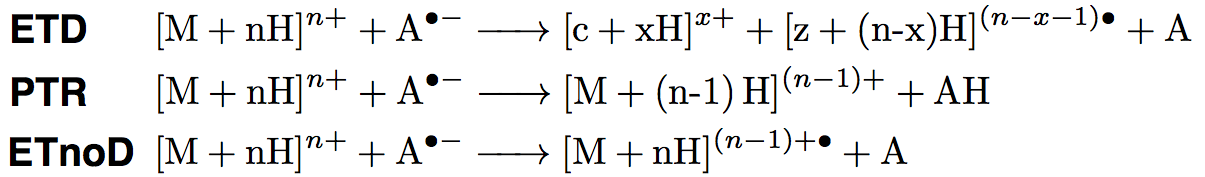
\includegraphics[width=.8\textwidth]{reactions.png}
                \caption{Chemical formulas of presumed ion-ion reactions. During the ETD a backbone bond between the
                \ce{C_\alpha} and \ce{N_\alpha} atoms is severed resulting in $c$ and $z$ ions. During the PTR, the anion cleaves one of protons that charged the precursor cation. During ETnoD, the radical is transfered from the anion onto the cation thereby reducing its charge.}\label{img::reactions}
        \end{figure}

        The appearance of the ETnoD fragments in the experimental data can be linked to the folding of proteins: although the covalent bond that kept the two fragments together was severed, noncovalent interactions keep them from parting \cite{LermyteJASMS2014,Lermyte2016}. In all of the above reactions the net charge on a protein reduces by one. Also, the mass of the radical can be neglected, given that most modern instruments do not resolve it. As a result, ETnoD products are heavier than PTR products and can be distinguished using mass spectrometry. Cations can undergo several reaction events while getting to the vicinity of different anions. However, so-called internal fragments of proteins (i.e. resulting from two backbone cleavage events) are usually not observed, suggesting that double ETD scarcely ever occurs. On the other hand, there is a lot of evidence of multiple ETnoD and PTR \cite{LermyteJASMS2015}.


\textbf{Related research.}
        The model we present is an extension to the approach presented by \cite{Gambin2010} that investigates proteolytic degradation induced by the exopeptidase enzyme. The authors use a Dynamic Stochastic Petri Net, DSPN, to model the behaviour of that system. A particular feature of the studied phenomenon is that the enzymatic cleavage of proteins cannot be reversed, i.e. proteins do not merge back into more complex molecules. This leads to a simplfied dynamics on the population level, as the average numbers of proteins at a given time can be obtained by solving a system of recursively dependent ordinary differential equations. The authors present an elegant dynamic algorithm for the retrieval of these quantities given some initial values of parameters. Then, the parameters are optimized in a way to minimize the difference between the calculated averages and the actual experimental data, obtained in a LC-MS experiment. This nonlinear least-squares optimization is performed using the BFGS algorithm.

        \todo[inline]{Prediction of Low-Energy Collision-Induced Dissociation Spectra of Peptides.}

\textbf{Our contribution.}
        We adjust the approach taken by \cite{Gambin2010} to the ETD setting. To study these reactions in detail, we have conducted controlled experiments on highly purified compounds. The identity of the precursor ion and all fragments obtained given a set of possible reaction is known and the quantities of these fragments can be established, approximately and up to proporionality factor, using our in-house developed identification tool called MassTodon \cite{LermyteIJMS2015,Lermyte2016}. Given a mass spectrum, MassTodon outputs lists of reaction products together with their estimated intensities, joining the intensitities of peaks coming from the same fragments and performing additional deconvolution when the source of ions cannot be uniquely determined. The obtained information is more compact, but still not easy to interpret: the number of possible fragments is usually linear in the lenght of the amino acid sequence and quadratic in the number of charge. The retrieveable data can be presented as a point in such highly dimensional space.

        The method we propose massively reduces this dimensionality. It is natural to assume that the resulting spectra are produced as an outcome of some stochastic chemical process governed by the intensities of these reactions. A process described by a small number of parameters can be more easily visualised and thus -- more easily understood. Low-dimensional representation of spectra considerably simplifies both the comparison of the spectra obtained from the instrument under different experimental settings and the comparison of spectra coming from different instruments.

\textbf{Organisation of the paper.}
        First, we introduce the theoretical considerations behind our model. Then, we describe the collection of data, both experimental and in silico, used to assess the quality of the model. Then, we describe the performance of the model and finally we sketch existing problems and possible extensions for the future work.

\section{Formal model of the ETD reaction}
        We model the ETD with a \textit{Dynamic Stochastic Petri Net}, DSPN. A \textit{Petri Net} is a bipartite directed graph with two types of nodes, called places and transitions\cite{Petri2008}. In the context of ETD, places correspond to cations that are substrates or products of the studied reactions, and transitions correspond to reactions that can occur in the chemical process, see Fig.~\ref{img::petrinet}.

        \begin{figure}[th]
                \center
                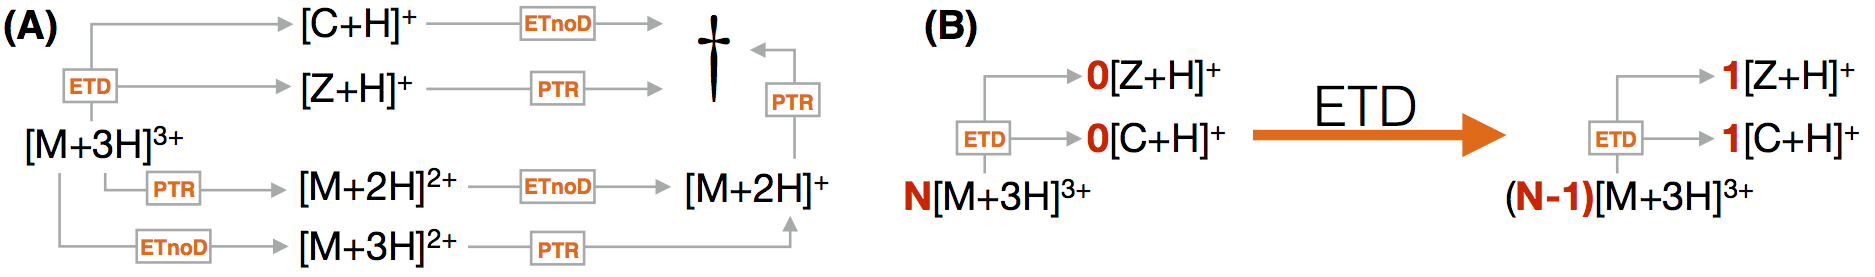
\includegraphics[width=\textwidth]{petrinet.png}
                \caption{A simplified \textit{Dynamic Stochastic Petri Net} of the ETD process. Chemical formulas (in black) correspond to places and names of reactions (in orange) -- to transitions. The dagger in (A) symbolizes a special state, called the \textit{cementary}. It is where the molecules introduced to the intrument but never observed, such as those that lost their charge or the inner fragments, end up. The graph serves as a board for tokens, whose counts are plotted in red in panel (B). Tokens can be found in places. If a reaction happens, one token from its source disappears and product tokens appear: one in case of ETnoD and PTR, two in case of ETD (that fragments into two precise fragments $c$ and $z$), as seen in (B). For a transition to take place, the number of substrate tokens must be greater than zero.}\label{img::petrinet}
        \end{figure}

        In the current set up, each place u can be uniquely described by: (1) the sequence of amino acids $s$, (2) the charge of the cation $q$, and (3) the number of protons $g$ that have been paired with electrons, so that $u = (s,q,g)$. Introduction of g is necessitated by the ETnoD reaction: each time it occurs an electron passes from the anion to the cation, reducing the charge of the cation without significantly modifying its mass. Remembering how many times this occured is necessary to correctly calculate the mass of cation. A special place is considered, the cementary, stores the molecules that cannot be observed in the experiment, such as cations that lost their charge or the inner fragments.

        Places are filled with tokens that represent the cations inside the instrument.  We denote the number of tokens at place u by xu. We call the collection of all such counts a state $x=(x_u)$. Given a state x the system can evolve to another state following one of possible transtions, like in Fig.~\ref{img::petrinet}(B).

        We investigate $L+2$ types of transitions, where $L$ is the number of amino acids of the protein under study minus the number of prolines that ETD cannot fragment. Two of them correspond to ETnoD and PTR reactions that change one substrate into one product. The remaining $L$ reactions are fragmentations along the backbone sequence, resulting in the $c$ and $z$ fragment ions.

        A DSPN is a \textit{Petri Net} where transitions are random and take place in random moments of time. Here, time is modelled as an interval ranging from $0$ -- the beginning of the process, to $1$ -- the moment of observation. In such setting, one can investigate how probable is it for the process $X$ to end up in state $x$ at a given time $t$. We denote that probability by $p_x^t$. The derivate of this quantity follows the master equation, $\dot{p}_x^t = \sum_{y\not=x} p_y^t Q_{yx} - p_x^t \sum_{y\not=x} Q_{xy},$ where $Q_{xy}$ is the intensity of the jump from state $x$ to $y$. The intensity equals $0$ if $y$ cannot be reached from $x$ by means of one reaction $R$. Otherwise, the intensity is assumed to be proportional to the number of the substrate molecules, $Q_{xy}=c_R x_{s_R}$,  where $c_R$ depends on the type of reaction and is explained in detail below.

        The average numbers of cations at that place $u$ is $E_u^t= \sum_x x_up_x^t$. At $t=0$, the process is not random: all tokens can be found only in the precursor node with maximal charge state, a place we call the root, or $r$. Thus, $E_r^0=N$ and $E_u^0=0$ if $u_0$. Later in time, the averages evolve according to $\dot E_u^t=\sum_x x_u \sum_{y\not=x} p_y^t Q_{yx} -\sum_x x_u p_x^t \sum_{y\not=x} Q_{xy}$. The double sums iterate over tuples $(x,y)$ or $(y,x)$ that correspond to reactions that change the first state to another by moving tokens. One can neglect states that cannot be obtained from other states, as then the intensity $Q_{xy}$ equals zero.
        This, and the asumption on the form of intensity, $Q_{xy}=c_Rx_{s_R}$, leads to $\dot E_u^t = \sum_R cR \left[ \sum_{x:x=Ry}  x_u (x_{s_R}+1) p_{R^{-1}x}^t- \sum_{x} x_u x_{s_R} p_x^t \right]$.
        Observe that for a given $R$,
                $$\sum_{x:x=Ry} x_u (x_{s_R}+1) p_{R^{-1}x}^t = \sum_{y}  (Ry)_u y_{s_R} p_y^t = \sum_x (Rx)_u x_{s_R} p_x^t,$$
        as we can restate the sums in terms of states from before transtion $R$ and retag $y$ for $x$. Thus, $\dot E_u^t = \sum_R c_R \sum_x   \left[(Rx)_u-x_u \right] x_{s_R} p_x^t$. The term $\left[(Rx)_u-x_u\right]$ equals $1$ if place $u$ is a product of reaction $R$, $-1$ for substrate, and $0$ otherwise. Therefore, it is a value dependent on $R$ and not on particular state $x$. Denote it by $K_R$. Then
                $$\dot E_u^t = \sum_R c_R K_R \sum_x x_{s_R} p_x^t = \sum_R c_R K_R E_{s_R}^t = \sum_{R:u\in P_R} c_R E_{s_R}^t - E_u^t \sum_{R: u=s_R}c_R,$$
        where $P_R$ are the products of reaction $R$. The inflow of molecules in place $u$ is proportional to the average numbers of the parent molecules of $u$ in the Petri Net. Their proportionality constants are equal to reaction intensities. The outflow depends on types of reactions that lead out of this place. In the Petri Net we consider, at most one transition can lead from one place to another. We can rewrite the above formula to underline the dependence of the average at place $u$ upon their parent places $v$, $ \dot E_u^t = \sum_{v\rightarrow u} \lambda_{vu} E_v^t - \lambda_{uu}E_u^t.$
        This system of ODEs is recursive and can be solved from the root $r$ downwards. For the root, $\dot E_r^t=-\lambda_{rr} E_r^t$, so that function $E_r^t= Ne^{-\lambda_{rr}t}$ solves it. This begins the recursion. Say that one computed all solutions that are parent of $u$. The form of the corresponding functions, $E_v^t$, is then known; denote them by $f_{>u}$. We assume that $r_u$. Thus, $\dot E_u^t=f_{>u}(t)-\lambda_{uu} E_u^t$. Given that $E_u^0=0$ for all $u_r$, the solution to this equation is, by straightforward integration, $E_u^t=e^{-\lambda_{uu}t} \int_0^t e^{\lambda_{uu}s} f_{>u}(s)ds$.
        Consider that $u$ is one of the sons of root $r$: plug $f_{>u}(s)=E_r^s$ to obtain $E_u^t= \frac{N}{\lambda_{rr}-\lambda_{uu}}(e{-\lambda_{uu}t}-e^{-\lambda_{rr}t})$. Similarly, one can prove that the general solution is $E_u^t=\sum_{v>u}b_{vu}e{-\lambda_{vv}t}-b_{uu}e^{-\lambda_{uu}t}$, where $b_{vu}= \frac{1}{\lambda_{uu}-\lambda_{vv}} \sum_{w: v\geq w \rightarrow u} \lambda_{wu}b_{vw}$ and  $b_{uu}=-\sum_v b_{vu}.$
        This holds only when $\lambda_{vv}\not=\lambda_{uu}$, which is true as shown below.

\section{Materials and Methods}
        \textbf{Simulations} Numerical simulations of ETD reaction were performed to verify the validity of the fitting procedure. At the onset of the simulation, for each peptide a given number of protons was placed randomly on basic amino acids, simulating the electrospray ionization of the peptide. Then, the reaction pathway of single molecules was simulated using standard methods for continuous-time markov jump processes\cite{Gillespie1977}, with assumption that each molecule reacts independently of other molecules. Finally, the obtained results for single molecules were combined together to get the state of the whole sample after given reaction time. Uniform cleavage of peptide bonds, with exception to the $N$-terminal bond of proline, was assumed during all simulations.

        To further analyze the robustness of the fitting procedure to noisy or missing data, we have added gaussian noise to the peak intensities and randomly removed a given proportion of peaks. The standard deviation of noise was proportional to the peak height.

        \textbf{Experimental data.} Substance P (Sigma S6883, 1.4 kDa) was dissolved at a concentration of 4 $\mu$M in water/acetonitrile v/v 50/50 and 1\% formic acid added. Approximately 5 $\mu$L of this solution was transferred to a gold-coated glass capillary prepared in-house and infused into the Synapt G2 mass spectrometer (Waters, Wilmslow, UK) using the nanoflow version of the Z-spray ion source, with a capillary voltage of 1.2 – 1.6 kV, minimal (<0.2 bar) nanoflow gas pressure, a backing pressure of 2.4 mbar and a source pressure of 1.6e-3 mbar. In ETD mode, reagent (1,4-dicyanobenzene) vapor is carried by a nitrogen flow at room temperature to the glow discharge needle located between the sampling cone and extraction cone, where radical anions are generated. The polarity of the ion optics up to and including the entrance of the trap cell is continuously switched, and after filling the T-wave trap cell with ETD reagent for 0.1 s, it is trapped there and allowed to interact for 1.0 s with the nano-ESI generated analyte cations, before the cycle starts again. Cation precursors and reaction products are axially propelled through the ETD reagent ‘‘cloud’’ in the trap cell by means of a travelling wave, the amplitude (‘height’) and velocity of which determine the extent and time of ion–ion interaction. The glow discharge was tuned to provide a signal of approximately 2e6 reagent counts per second (make-up gas flow 35 mL/min, discharge current 20 $\mu$A). Instrument settings were as follows: sampling cone 60 V, extraction cone 2 V, trap pressure 6.2e-2 mbar, trap collision energy 4 V, trap DC bias 8 V, transfer pressure 1.2e-2 mbar. The instrument was operated in Sensitivity mode and fitted with a 32 K quadrupole. For relative peak intensity measurements, the spectrum was smoothed (2x three-channel Savitsky-Golay method) and centered using MassLynx (version 4.1).

        \section{Results}

        \textbf{In silico.} We have performed \textit{in silico} tests to assess the correctness and robustness of our estimation methods in a fully controlled setting. On simulated data without noise, the model was able to predict the reaction intensities with high accuracy even for small numbers of molecules in the sample. We have fitted the model to several simulation settings, corresponding to theoretically predicted average loss of 0 to 6 charges during the reaction time (where an average loss of 6 charges means that the vast majority of molecules will be fully neutralized). The obtained estimates were unbiased, with low variance. The results of estimation are summed up in Fig.\todo{add fig.}

        The fitting procedure turned out to be fairly robust against moderate noise and missing data. We have fitted the model to simulated datasets with noise for constant reaction intensities of ETD, PTR and ETnoD equal to $0.06, 0.05$ and $0.09$, respectively. The intensities were chosen to represent an experimental setting in which our model gives good prediction of experimental results and is therefore assumed to be based on assumptions valid in this experimental regime (Wave Height $= 1.5$, Wave Velocity $= 10$). This set of intensities corresponds to the loss of less than one charge on average (16\% neutralized molecules).

        The simulated datasets were then \textit{corrupted} with various proportions of missing data without noise, various noise intensities without data loss, and various proportions of missing data for noise standard deviation set to one fifth of the peak height. For each setting, $100$ replications were performed, and standard euclidean distance between true and estimated intensities was computed. The results are summed up in Fig.\todo{add fig.}

        \textbf{Fitting experimental data.}
        The model has been fitted to Substance P spectra, described in \textit{Materials and Methods}. After fitting the model to the data, the validity of the model was further investigated by computing the percentage of the experimental spectrum explained by the theoretically predicted spectrum. The percentage of explanation was defined as the common part of a theoretical and experimental spectrum. For an additional measure of overall reaction intensity, the percentages of neutralized molecules were computed from the predicted spectra.

	We have observed missing data in our experimental spectra, as some peptide fragments were missing their corresponding counterparts in several spectra. To account for this, an adjusted explanation percentage was also computed, where theoretical peaks corresponding to unobserved experimental peaks were assumed to be fully explanatory.
	The typical values of explanation percentage were between 73\% and 98\% without adjustment for missing data, and between 86\% and 99\% with the adjustment. Taking into account the fact that only the average intensities were computed, i.e. disregarding their dependence on the peptide sequence and conformation, this result is very optimistic.
	The predicted percentage of neutralized molecules ranged from <1\% to 99\%.  A strong negative correlation (-0.73) between percentage of neutralized molecules and percentage of spectrum explanation was found. This indicates that our model is valid mostly in the regime of small and moderate reaction intensities, and performs worse in more harsh experimental conditions. Accordingly, the typical values of explanation percentage for spectra in which there was less than 50\% of fully neutralized molecules are between 83\% and 99\% (without adjustment for missing data).

\section{Discussion}
        Analyzing the experimental data using mathematical tools allows to gain more insight into the nature of the chemical processes and to predict their outcome. Our model proved useful for explaining and investigating the Electron Transfer Dissociation reaction for moderate experimental conditions. We were able to infer the ratios of ETD and side reaction intensities, investigate the uniformity of peptide bond cleavage and compute the percentage of neutralized molecules.

        The spectra in our experimental dataset correspond to various values of wave height, controlling the extent of interactions between the analyte and the reagent, and wave velocity, controlling the reaction time. Therefore, smaller wave heights cause more reactions. On the other hand, the influence of wave velocity value on reaction intensity is more complicated. Low wave velocities promote longer reaction times, thus increasing number of reactions. However, for very high wave velocities, the energy transfer rate from the wave to the ions drop, again increasing the reaction intensity. Thus, reaction intensity is the lowest for a specific value of wave velocity and increases as this parameter changes in any direction. This behaviour is indeed observed in the percentages of neutralized molecules predicted from the reaction intensity estimates. Overall, we are able to control the harshness of the reaction conditions by changing the values of wave velocity and wave height.

        By fitting our model to spectra obtained with different instrumental settings, we have investigated the range in which our assumptions on the chemical nature of ETD seem to be appropriate. For wave heights from 0.4 to 1.5 and wave velocity 300, the model allows to explain over 85\% of the spectrum; For various wave velocity values and wave height 1.5 we get good prediction in the intervals from 15 to 700, corresponding to moderate reaction intensities (less than 2\% neutralized molecules). The high explanation percentages for high wave velocities (over 2750) are not to be trusted, as they correspond to over 99\% neutralized molecules.

        For wave height values less than 0.4 and/or wave velocity greater than 700 the performance of our model drops, indicating that there are some other chemical phenomena that play an important role. From the manual inspection of the experimental spectra and comparison with the theoretically predicted ones, we have noticed that for the precursor sequence, there is much more ETnoD products than our model predicts, while for the fragment sequences it is converse, and PTR products dominate. This suggests significant difference in PTR/ETnoD ratio for different molecules, which may be due to their conformation, as suggested by \cite{Lermyte2016}. The difference is less drastic in the moderate experimental conditions, though still visible.

	The obtained results are promising for future work, as even for the worst cases over 65\% of the experimental spectrum could be explained by our model. As a tool for estimating ETD, PTR and ETnoD intensities averaged over all molecules, this model is a valuable reference for more complex ones that will include the changing PTR/ETnoD ratios for different molecules; It will also be used to correlate the instrumental settings with average reaction intensities to facilitate predicting the proper experimental conditions to obtain desired results. The percentage of neutralized molecules predicted from the observable part of the spectrum can also be used to infer the initial amount of analyte in the sample. Overall, there are vast possibilities for mathematical modelling in the study of the Electron Transfer Dissociation reaction, and in the field of mass spectrometry in general.

% \bibliographystyle{splncsnat.bst}
\bibliographystyle{splncs03.bst}
{\footnotesize\bibliography{ISBRA_pubs}}

\end{document}
